%%%%%%%%%%%%%%%%%%%%%%%%%%%%%%%%%%%%%%%%%%%%%%%%%%%%%%%%
%%%%%%                                            %%%%%%
%%%                                                  %%%
%      Modèle de Rapport.                              %
%               Par Matthieu Maury                     %
%                                                      %
%%%                                                  %%%
%%%%%%                                            %%%%%%
%%%%%%%%%%%%%%%%%%%%%%%%%%%%%%%%%%%%%%%%%%%%%%%%%%%%%%%%

\documentclass[10pt, a4paper]{report}

%%%%%%%%%%%%%%%%%%%%%%%%%%%%%%%%%%%%%%%%%%%%%%%%%%%%%%%%
%% Package essentiel
\usepackage[greek,english]{babel}
\usepackage[T1]{fontenc}
\usepackage{ucs}
\usepackage[utf8x]{inputenc}
\usepackage[top=2.6cm,bottom=2.6cm,right=2.1cm,left=2.1cm]{geometry}
\usepackage{float}

%%%%%%%%%%%%%%%%%%%%%%%%%%%%%%%%%%%%%%%%%%%%%%%%%%%%%%%%
%% Package optionnel
\usepackage{enumerate}
\usepackage{graphicx}
\usepackage{tabularx}
\usepackage{setspace}
\usepackage[dvips]{pstricks}
\usepackage{pstricks-add}
\usepackage{color}
\usepackage{xcolor}
\usepackage{epsfig}
\usepackage{pst-grad} % For gradients
\usepackage{pst-plot} % For axes
\usepackage{amsmath}
\usepackage{amsfonts}
\usepackage{amssymb}
\usepackage{amsxtra}
\usepackage{mathrsfs}
\usepackage{framed}
%\usepackage[framed, thmmarks, amsmath]{ntheorem}
\usepackage{verbatim}
\usepackage{moreverb}
\usepackage{fancyhdr}
\usepackage{url}
\usepackage{listings}
%\usepackage{hyperlinks}
\usepackage{lettrine}

%%%%%%%%%%%%%%%%%%%%%%%%%%%%%%%%%%%%%%%%%%%%%%%%%%%%%%%%
%%%%%%                                            %%%%%%
%%         Configuration de la mise en page           %%
%%%%%                                              %%%%%
%%%%%%%%%%%%%%%%%%%%%%%%%%%%%%%%%%%%%%%%%%%%%%%%%%%%%%%%

%%%%%%%%%%%%%%%%%%%%%%%%%%%%%%%%%%%%%%%%%%%%%%%%%%%%%%%%
%% Profondeur du sommaire
\setcounter{secnumdepth}{4}
\setcounter{tocdepth}{4}

%%%%%%%%%%%%%%%%%%%%%%%%%%%%%%%%%%%%%%%%%%%%%%%%%%%%%%%%
%% Configuration des chapitres
\makeatletter
\def\@makechapterhead#1{%
  \vspace*{50\p@}%
  {\parindent \z@ \raggedright \normalfont
    \interlinepenalty\@M
    \Huge \bfseries\thechapter.\quad#1\par\nobreak
    \vskip 20\p@
  }}
\makeatother

%%%%%%%%%%%%%%%%%%%%%%%%%%%%%%%%%%%%%%%%%%%%%%%%%%%%%%%%
%%%%%%                                            %%%%%%
%%                Début du Document                   %%
%%%%%                                              %%%%%
%%%%%%%%%%%%%%%%%%%%%%%%%%%%%%%%%%%%%%%%%%%%%%%%%%%%%%%%


\lstset{tabsize=3, inputencoding=utf8x, extendedchars=\true, language=C}

%% Symboles des ensembles
\newcommand{\R}{\ensuremath{\mathbb{R}} }
\newcommand{\N}{\ensuremath{\mathbb{N}} }
\newcommand{\Z}{\ensuremath{\mathbb{Z}} }
\newcommand{\Q}{\ensuremath{\mathbb{Q}} }
\newcommand{\C}{\ensuremath{\mathbb{C}} }
\newcommand{\U}{\ensuremath{\mathbb{U}} }
\newcommand{\K}{\ensuremath{\mathbb{K}} }

%% Symboles mathématique
\newcommand{\spi}{\ensuremath{\Pi} } %Pi
\newcommand{\sqqs}{\ensuremath{\forall} } %quelque soit
\newcommand{\sex}{\ensuremath{\exists} } %il existe
\newcommand{\snex}{\ensuremath{\nexists} }
\newcommand{\simpld}{\ensuremath{\Rightarrow} } %implique vers la droite
\newcommand{\simplg}{\ensuremath{\Leftarrow} } %implque vers la gauche
\newcommand{\sequ}{\ensuremath{\Leftrightarrow} }
\newcommand{\sand}{\ensuremath{\wedge} }
\newcommand{\sou}{\ensuremath{\vee} }
\newcommand{\smneg}{\ensuremath{\neg} }
\newcommand{\snimpld}{\ensuremath{\nRightarrow} } %implique vers la droite
\newcommand{\snimplg}{\ensuremath{\nLeftarrow} } %implque vers la gauche
\newcommand{\snequ}{\ensuremath{\nLeftrightarrow} }
\newcommand{\sinclut}{\ensuremath{\in} }
\newcommand{\sninclut}{\ensuremath{\notin} }
\newcommand{\sposd}{\ensuremath{\owns} }
\newcommand{\ssups}{\ensuremath{\supset} }
\newcommand{\snsups}{\ensuremath{\nsupset} }
\newcommand{\ssubs}{\ensuremath{\subset} }
\newcommand{\ssubeq}{\ensuremath{\subseteq} }
\newcommand{\ssupeq}{\ensuremath{\supseteq} }
\newcommand{\snsubeq}{\ensuremath{\nsubseteq} }
\newcommand{\snsupeq}{\ensuremath{\nsupseteq} }
\newcommand{\sneg}{\ensuremath{\neq} }
\newcommand{\saprox}{\ensuremath{\approx} }
\newcommand{\ssim}{\ensuremath{\sim} }
\newcommand{\scompl}[2]{\ensuremath{\complement_{#1}{#2}} }
\newcommand{\sunion}{\ensuremath{\cup} }
\newcommand{\sinters}{\ensuremath{\cap} }
\newcommand{\sx}{\ensuremath{\times} }
\newcommand{\svide}{\ensuremath{\emptyset} }
\newcommand{\Pa}{\ensuremath{\mathcal{P}} }
\newcommand{\lra}{\ensuremath{\longrightarrow}}
\newcommand{\rond}{\ensuremath{\circ} }
\newcommand{\frestric}[2]{\ensuremath{#1|_{#2}} }
\newcommand{\sbar}[1]{\ensuremath{\overline{#1}}}
\newcommand{\si}{\ensuremath{\imath}}
\newcommand{\zl}[1]{\ensuremath{\mathscr{#1}}}
\newcommand{\stimes}{\ensuremath{\times}}
\newcommand{\classe}[1]{\ensuremath{\overset{\bullet}{#1}}}


\begin{document}

%%%%%%%%%%%%%%%%%%%%%%%%%%%%%%%%%%%%%%%%%%%%%%%%%%%%%%%%
%% Inclusion de la page de titre
\pagestyle{fancy}
\renewcommand{\sectionmark}[1]{\markright{\thesection\ #1}}
\renewcommand{\footrulewidth}{0pt}
\renewcommand{\headrulewidth}{0pt}
\fancyhead{} % clear all header fields
\fancyfoot{} % clear all footer fields
\fancyfoot[LO,RE]{\textit{University year 2009-2010}}
\fancyfoot[LE,RO]{\textit{Written with \LaTeX}}

\begin{tabularx}{17cm}{Xr}
  \begin{tabular}{ll}
    Yohann Teston & 881003-P792\\
    \url{yohann.teston@free.fr} &\\
	Matthieu Maury & 860928-P210\\
	\url{mayeu.tik@gmail.com} & \\
  \end{tabular} 

  &
  
  \begin{tabular}{r}
    
\includegraphics[width=5cm]{pic/logoupp.eps} \\
    \textit{Department of Information Technology} \\
  \end{tabular}
\end{tabularx}

\vspace{6cm}

\begin{center}
  \textbf{ {\Huge Programming of parallel computers}}\\[0.5em]{\huge Lab 2 - Pthreads}
\end{center}

\begin{center}
  \today
\end{center}


\newpage


\thispagestyle{empty}
%\input{resume}

\renewcommand{\footrulewidth}{0.5pt}
\renewcommand{\headrulewidth}{0.5pt}
\fancyhead{} % clear all header fields
\fancyhead[RE,LO]{Programming of parallel computers - Lab 2 - Pthreads}


\fancyhead[RO,LE]{\rightmark}

\fancyfoot{} % clear all footer fields
\fancyfoot[LO,RE]{Matthieu Maury \& Yohann Teston}
\fancyfoot[LE,RO]{\thepage}

%Redéfinition du style fancy - plain, utilisé pour les pages de nouveau chapitre
%Le style par défaut est un style plain
\fancypagestyle{plain}{
    \fancyhf{}
    \renewcommand{\headrulewidth}{0pt}

    %Définition des headers identiques à une page normale
    \fancyfoot[LO,RE]{Matthieu Maury \& Yohann Teston}
    \fancyfoot[LE,RO]{\thepage}
}

\tableofcontents

%\listoffigures

%\newpage

%\doublespacing
\onehalfspacing
\chapter{Compile and run Pthreads programs}

As expected, running the hello program results in several \textit{Hello World!} being printer, one for each processor we are running on.

After modification of the program, we have the following result:

\verbatiminput{file/q1.1}

We can see that there is no pre-defined order between the threads because the order of the messages changes. This is due to the thread scheduler. So, there is no way to tell which one will start first or in which order the result will appear.

The second program use a struct to pass more argument to the thread. After the modification we got the following output:

\verbatiminput{file/q1.2}


\chapter{Global and local data}

We have the following output:
\verbatiminput{file/q2}

We can see that the value in the array is not the same depending wich thread print it. This is because all the thread won't run at the same time. So if a thread print the array befaure another write in it, we will not be able to see the modification.

\chapter{Collective communication, global data}

If the thread are joinable the main program will wait in the \verb+pthread_join+ function that all the thread finish their work:

\verbatiminput{file/q3.1}

Now if we set the thread as detachable thread, we see that main finish his work, and wait for the thread just before exiting:

\verbatiminput{file/q3.2}

Finally, by removing \verb+pthread_exit+ from the main we see that the program exit without waiting for the thread:

\verbatiminput{file/q3.3}

\chapter{Introduction to Pthreads}

\section{Mutex variables}

If a mutex is not used to protect the access to the shared variable $sum$, the result will not be reliable. Indeed, race conditions will appear and modifications will then be lost. A race condition appear when several threads access the same memory space without protection. For example, a thread could read $sum$ in a register, modify it and be preempted just before writing it back. When this thread will be allocated the CPU again, it will then erase all modifications that could have happened meanwhile by storing its local value into the shared variable.

Mutexes are then indispensable when it comes to multithreading.

\section{Condition variables}

If the barrier is removed in the first program, there will be no synchronization between the threads. They will not wait for everyone to be done with the first printing and selfishly continue. The output will then look like that:
\begin{center}
	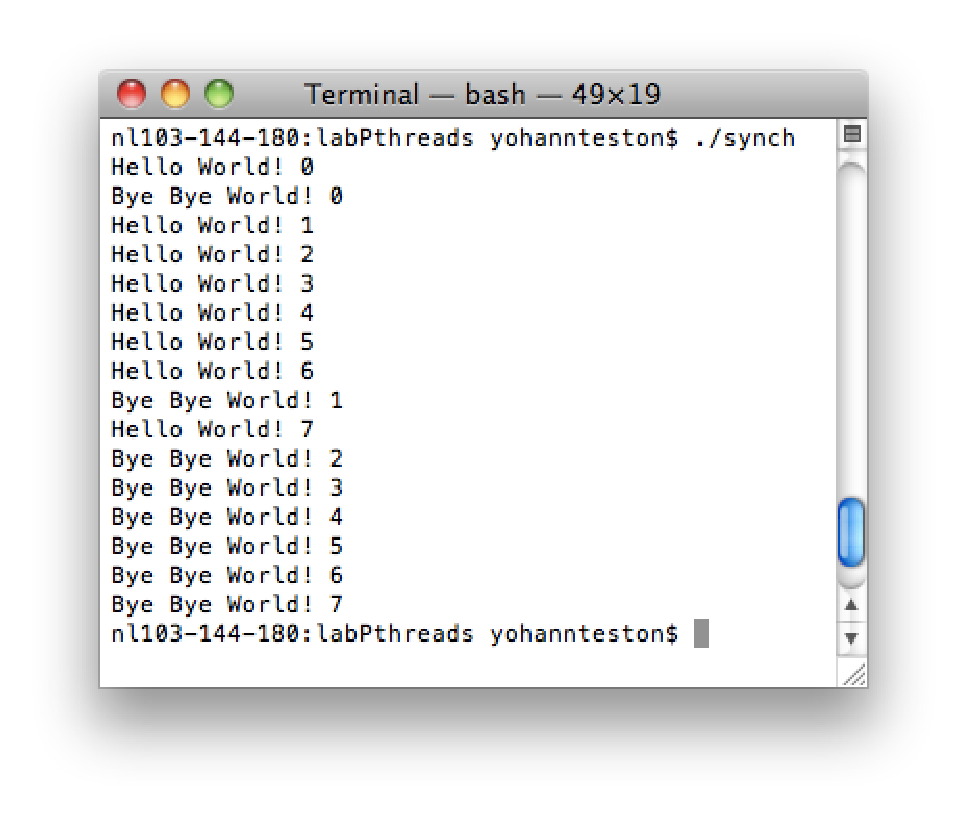
\includegraphics[width=\textwidth]{pic/q5.eps}
\end{center}


In \textit{spinwait.c}, the problem arises because the program does not load $state$'s value in a register for each test but do that once before the loop. So, when the last thread modifies $state$, its new value is not read by the other processes. Therefore, they keep spinning indefinitely. To avoid this, we have to make sure the compiler will generate a memory access each time $state$ is accessed. We can do that using the keyword $volatile$. We can then try again the program and see that everything works fine. 

\chapter{Examples}

\section{Pi}

The C code for this program is available in the appendix \ref{pi}. 

\section{PDE solver}

The graphs \ref{overlap} and \ref{synchro} show the speedup for both of the synchronization methods.

%\begin{figure}[!h]
 % \begin{center}
  %       \resizebox{160mm}{!}{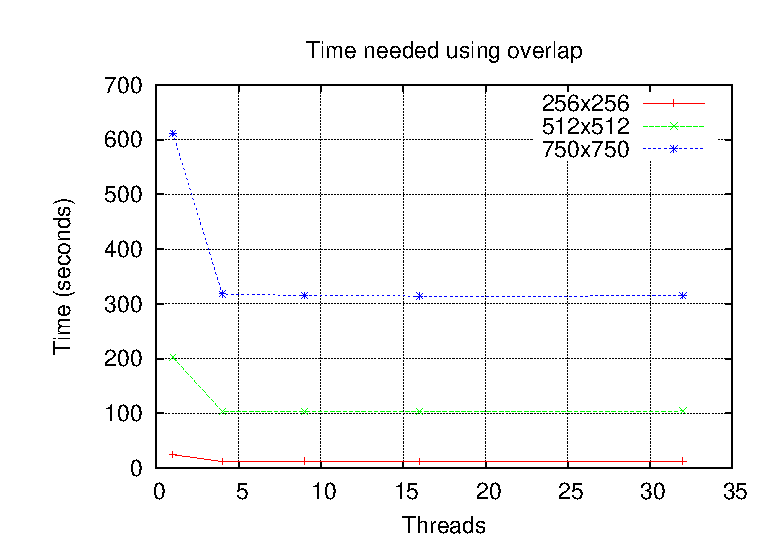
\includegraphics{pic/graph_over_time.eps}}
  %\end{center}
  %\caption{Time needed using overlap}
%\end{figure}

\begin{figure}[!h]
  \begin{center}
         \resizebox{160mm}{!}{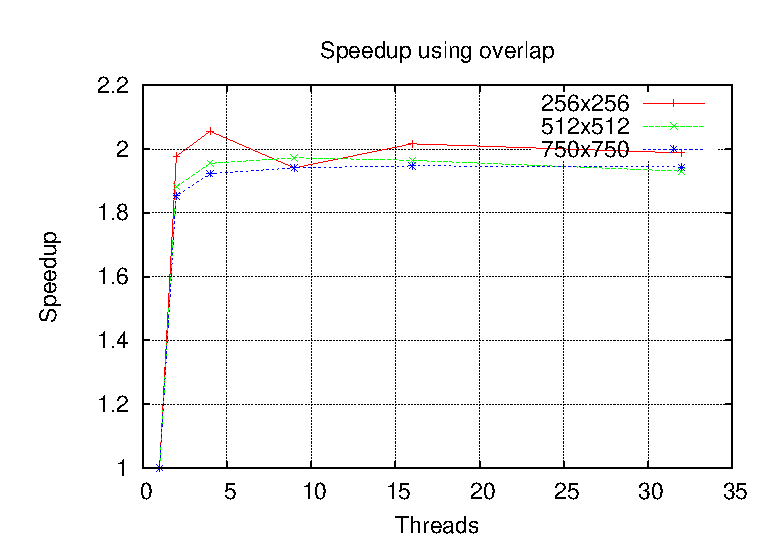
\includegraphics{pic/graph_over.eps}}
  \end{center}
  \caption{Speedup using overlap}
  \label{overlap}
\end{figure}

%\begin{figure}[!h]
 % \begin{center}
  %       \resizebox{160mm}{!}{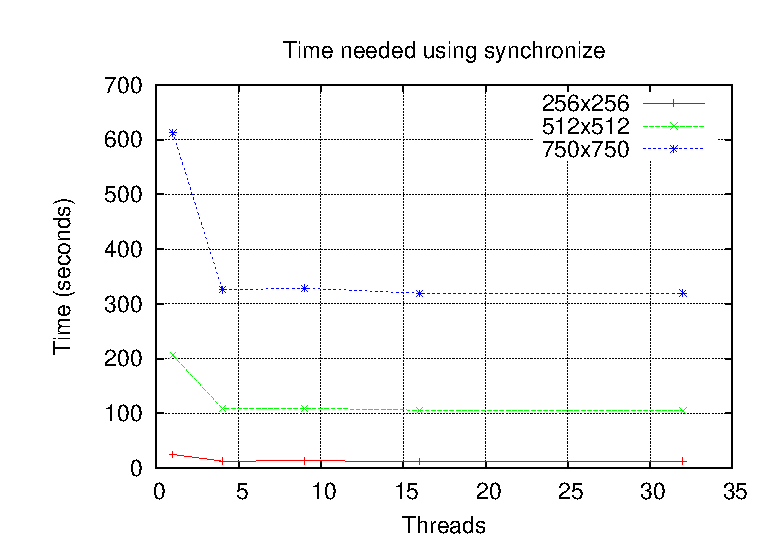
\includegraphics{pic/graph_synchro_time.eps}}
 % \end{center}
 % \caption{Time needed using synchronize}
%\end{figure}

\begin{figure}[!h]
  \begin{center}
         \resizebox{160mm}{!}{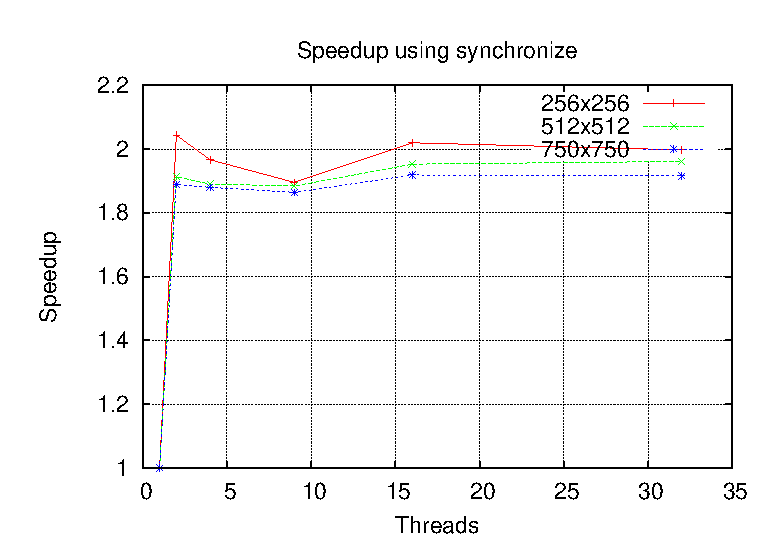
\includegraphics{pic/graph_synchro.eps}}
  \end{center}
  \caption{Speedup using synchronize}
  \label{synchro}
\end{figure}

As we can see in those pictures, the speedup remains the same for both of the methods. The speedup is only good during the first step, that is from 1 to 4 threads, and remains more or less the same because of the synchronization. Indeed, regardless of the method we choose, threads must be synchronized.

When several threads are used (from 2 to 32 in our example), the execution time does not change much. The only change that is worth notifying is the one that occurs when we go from 1 thread to 2 threads. At that time, the execution is basically divided by two. However, this cannot be said for the rest of the graph. This is because of synchronization. Indeed, using several threads increases performances but brings also the need to synchronize them. The time spent for this hinders the performances and creates some kind of lower bound the execution time cannot (around half of the time on one thread).

\chapter{Matrices multiplication}

The code of the non-optimized version of this program can be found in the appendix \ref{matmul} and that of the optimized version in the appendix \ref{matmulot}. 
The optimization done in the version is simply an inversion of the two inner loops used to perform the matrices multiplication. It optimizes the use of the cache and this is enough to speed the program up considerably.

The picture \ref{matmul} presents the results.

\begin{figure}[h]
  \begin{center}
         \resizebox{160mm}{!}{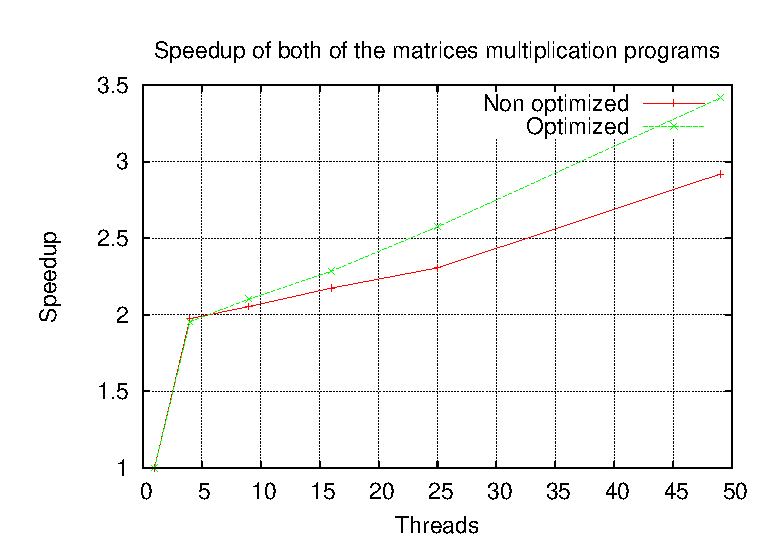
\includegraphics{pic/graph_matmul.eps}}
  \end{center}
  \caption{Speedup of both of the matrices multiplication programs}
  \label{matmul}
\end{figure}

As we can see on the diagram, performances are better with the cache optimisation of the second version. This shows the importance of knowing how data is stored in the computer and how to optimize the access to it.


\newpage
\setcounter{page}{1}
\pagenumbering{Roman}
\appendix
\chapter{$\pi$}

\lstinputlisting{../labPthreads/pi.c}
\label{pi}
\chapter{Matrices multiplication}

\section{Non-optimized code}
\label{matmul}
\lstinputlisting{../labPthreads/matmul.c}

\section{Optimized code}
\label{matmulot}
\lstinputlisting{../labPthreads/matmulot.c}



\end{document}
